\documentclass[a4paper,10pt]{report}

\usepackage{tikz}
\usetikzlibrary{shadows.blur}
\usetikzlibrary{shapes.symbols}

\usepackage{fancybox, graphicx}
\usepackage{hyperref}
\usepackage{amsmath}
\usepackage{amssymb}
\usepackage{xspace}
\pagestyle{headings}
%\usepackage[margin=1.2in]{geometry}
\usepackage[left=2cm, right=2cm, top=2.5cm, bottom=2cm]{geometry}
\usepackage{float}
\restylefloat{table}
\usepackage{listings}
\usepackage{color}
\definecolor{gray}{rgb}{0.4,0.4,0.4}
\definecolor{darkblue}{rgb}{0.0,0.0,0.58}
\definecolor{attributeColor}{rgb}{0.96,0.517,0.29}
\definecolor{darkgreen}{rgb}{0,.392,0}
\definecolor{stringColor}{rgb}{0.6,0.2,0}
\usepackage{array,multirow}
\usepackage{longtable}
\usepackage{cleveref}
\usepackage{bbding}
\crefname{section}{�}{��}
\Crefname{section}{�}{��}
\usepackage[utf8]{inputenc}
\usepackage{tablefootnote}
\usepackage{algorithmic}
\usepackage[modulo, pagewise]{lineno}
%\nolinenumbers
\usepackage{makecell}
\usepackage{multicol}
\usepackage{url}
\usepackage{verbatimbox}
\usepackage{xcolor}
\usepackage{cancel}

\usepackage{caption} 
\captionsetup[table]{skip=5pt}
\captionsetup[longtable]{skip=5pt}
\captionsetup[figure]{skip=1pt}

\usepackage{titlesec}
\titlespacing*{\subsection}{0pt}{1.5\baselineskip}{\baselineskip}

\usepackage[utf8]{inputenc}
\usepackage[english]{babel}
 
\newcounter{example}[section]
\newenvironment{example}[1][]{\refstepcounter{example}\par\medskip
   \textbf{Example~\theexample. #1} \rmfamily}{\medskip}
   
\newcounter{note}[section]
\newenvironment{note}[1][]{\refstepcounter{note}\par\medskip
   \textbf{Note~\thenote. #1} \rmfamily}{\medskip}
   
\newcommand{\myStartLine}{\par
  \kern8pt % space above the rules
  \hrule height 0.5pt
  \kern3pt % space below the rules
}
\newcommand{\myEndLine}{\par
  \kern3pt % space above the rules
  \hrule height 1.5pt
  \kern12pt % space below the rules
}

\newcommand{\HRule}{\rule{\linewidth}{0.5mm}}

\lstdefinelanguage{XML}
{
  basicstyle=\ttfamily\footnotesize,
  morestring=[b]",
  morestring=[s]{>}{<},
  moredelim=[s][\bfseries\color{darkblue}]{<}{\ },
  moredelim=[s][\bfseries\color{darkblue}]{</}{>},
  moredelim=[l][\bfseries\color{darkblue}]{/>},
  moredelim=[l][\bfseries\color{darkblue}]{>},
  morecomment=[s]{<?}{?>},
  morecomment=[s]{<![CDATA[}{]]>},
  moredelim=[s][\bfseries\color{darkgreen}]{<!--}{-->},
  commentstyle=\color{darkgreen},
  stringstyle=\color{stringColor},
  identifierstyle=\color{red},
  keywordstyle=\color{attributeColor},
  morekeywords={oid,columnId,columnIdRef,symbId,symbolType,op,columnNum,columnType,
  valueType,inputTarget,blkId,blkIdRef,symbIdRef,xmlns,version,type,VariableMapping,
  IndividualMapping,schemaLocation,xs,xsi,NONMEMdataSet,matrixType,opType,order,
  math,ct,ds,mdef,mstep,mml,un,name,definition,writtenVersion,id,inputType,oidRef,catId,
  length,default,vectorIndex,diagDefault,offDiagDefault,row,column,numbRows,numbCols,
  dataSymbol,modelSymbol,ordered,compartmentNo,compNo,ordered,linkFunction,varId,
  censoringType,dataSymbol,modelSymbol,MarkovOrder,deviationMatrixType,implementedBy,
  argument,admNumber,transformId,transformIdRef,catIdRef,headerType,rowNumber,
  toolName,dataCode,missingDataType,regressor,fixed,symbol,transform} % list your attributes here
}

\lstdefinelanguage{MLX} 
{
  basicstyle=\ttfamily\footnotesize,
  morestring=[b]",
  morestring=[s]{>}{<},
  moredelim=[s][\bfseries\color{darkblue}]{<}{\ },
  moredelim=[s][\bfseries\color{darkblue}]{</}{>},
  moredelim=[l][\bfseries\color{darkblue}]{/>},
  moredelim=[l][\bfseries\color{darkblue}]{>},
  morecomment=[s]{<?}{?>},
  morecomment=[s]{<!--}{-->},
  morecomment=[s]{<![CDATA[}{]]>},
  commentstyle=\color{darkgreen},
  stringstyle=\color{stringColor},
  identifierstyle=\color{black},
  keywordstyle=\color{attributeColor},
  morekeywords={dads} % list your attributes here
}

\lstdefinelanguage{NM}
{
  basicstyle=\sffamily\small,
  morestring=[b]",
  morestring=[s]{>}{<},
  moredelim=[is][\bfseries\color{red}]{[*}{*]},
  moredelim=[s][\bfseries\color{darkblue}]{<}{\ },
  moredelim=[s][\bfseries\color{darkblue}]{</}{>},
  moredelim=[l][\bfseries\color{darkblue}]{/>},
  moredelim=[l][\bfseries\color{darkblue}]{>},
  morecomment=[s]{<?}{?>},
  morecomment=[s]{<!--}{-->},
  morecomment=[s]{<![CDATA[}{]]>},
  commentstyle=\color{darkgreen},
  stringstyle=\color{stringColor},
  identifierstyle=\color{black},
  keywordstyle=\color{attributeColor},
  morekeywords={kjkj} % list your attributes here
}

\newcommand{\cellml}{CellML\xspace}
\newcommand{\sbml}{SBML\xspace}
\newcommand{\sedml}{SED-ML\xspace}
\newcommand{\mathml}{MathML\xspace}
\newcommand{\uncertml}{UncertML\xspace}
\newcommand{\pml}{PharmML\xspace}
\newcommand{\pharmml}{PharmML\xspace}
\newcommand{\xelem}[1]{\texttt{<#1>}\index{XML Element!\texttt{<#1>}}}
\newcommand{\xatt}[1]{\texttt{#1}\index{XML Attribute!\texttt{#1}}}

\begin{document}

%\begin{titlepage}
\begin{center}

% Upper part of the page. The '~' is needed because \\
% only works if a paragraph has started.

\includegraphics[width=0.35\textwidth]{./logo/ddmore_logo}~\\[1cm]

%\textsc{\LARGE }\\[1.5cm]
%
\textsc{\Large Technical Report}\\[0.5cm]

% Title
\HRule \\[0.4cm]
{ \huge \bfseries Negative Binomial \\[0.4cm] }

\HRule \\[1.5cm]

Maciej J \textsc{Swat}\\
EMBL-EBI


\vfill

% Bottom of the page
{\large \today \\}

\end{center}
\end{titlepage} 
%\begin{titlepage}
\begin{center}

% Upper part of the page. The '~' is needed because \\
% only works if a paragraph has started.

\includegraphics[width=0.35\textwidth]{./logo/ddmore_logo}~\\[1cm]

%\textsc{\LARGE }\\[1.5cm]
%
\textsc{\Large Technical Report}\\[0.5cm]

% Title
\HRule \\[0.4cm]
{ \huge \bfseries GNB Distribution Family \\[0.4cm] }

\HRule \\[1.5cm]

Maciej J \textsc{Swat}


\vfill

% Bottom of the page
{\large \today \\}

\end{center}
\end{titlepage} 
%\begin{titlepage}
\begin{center}

% Upper part of the page. The '~' is needed because \\
% only works if a paragraph has started.

\includegraphics[width=0.35\textwidth]{./logo/ddmore_logo}~\\[1cm]

%\textsc{\LARGE }\\[1.5cm]
%
\textsc{\Large Internal Release}\\[0.5cm]

% Title
\HRule \\[0.4cm]
{ \huge \bfseries Extensions in PharmML 0.7.1 \\[0.4cm] }

\HRule \\[1.5cm]

% Author and supervisor
\begin{minipage}{0.5\textwidth}
\begin{flushleft} \large
\emph{Authors:}\\
Maciej J \textsc{Swat}\\
%Pierre \textsc{Grenon}\\
%Florent \textsc{Yvon}\\
Sarala \textsc{Wimalaratne}\\
Niels Rode \textsc{Kristensen}\\
\end{flushleft}
\end{minipage}
%\begin{minipage}{0.4\textwidth}
%\begin{flushright} \large
%\emph{with contributions from:} \\
%%%Roberto \textsc{Bizzotto} \\
%Emmanuelle \textsc{Comets}\\
%Paolo \textsc{Magni}\\
%Lorenzo \textsc{Pasotti}\\
%Marc \textsc{Lavielle}
%%Nadia \textsc{Terranova}\\
%\end{flushright}
%\end{minipage}

\vfill
\begin{figure}[htb]
\centering
  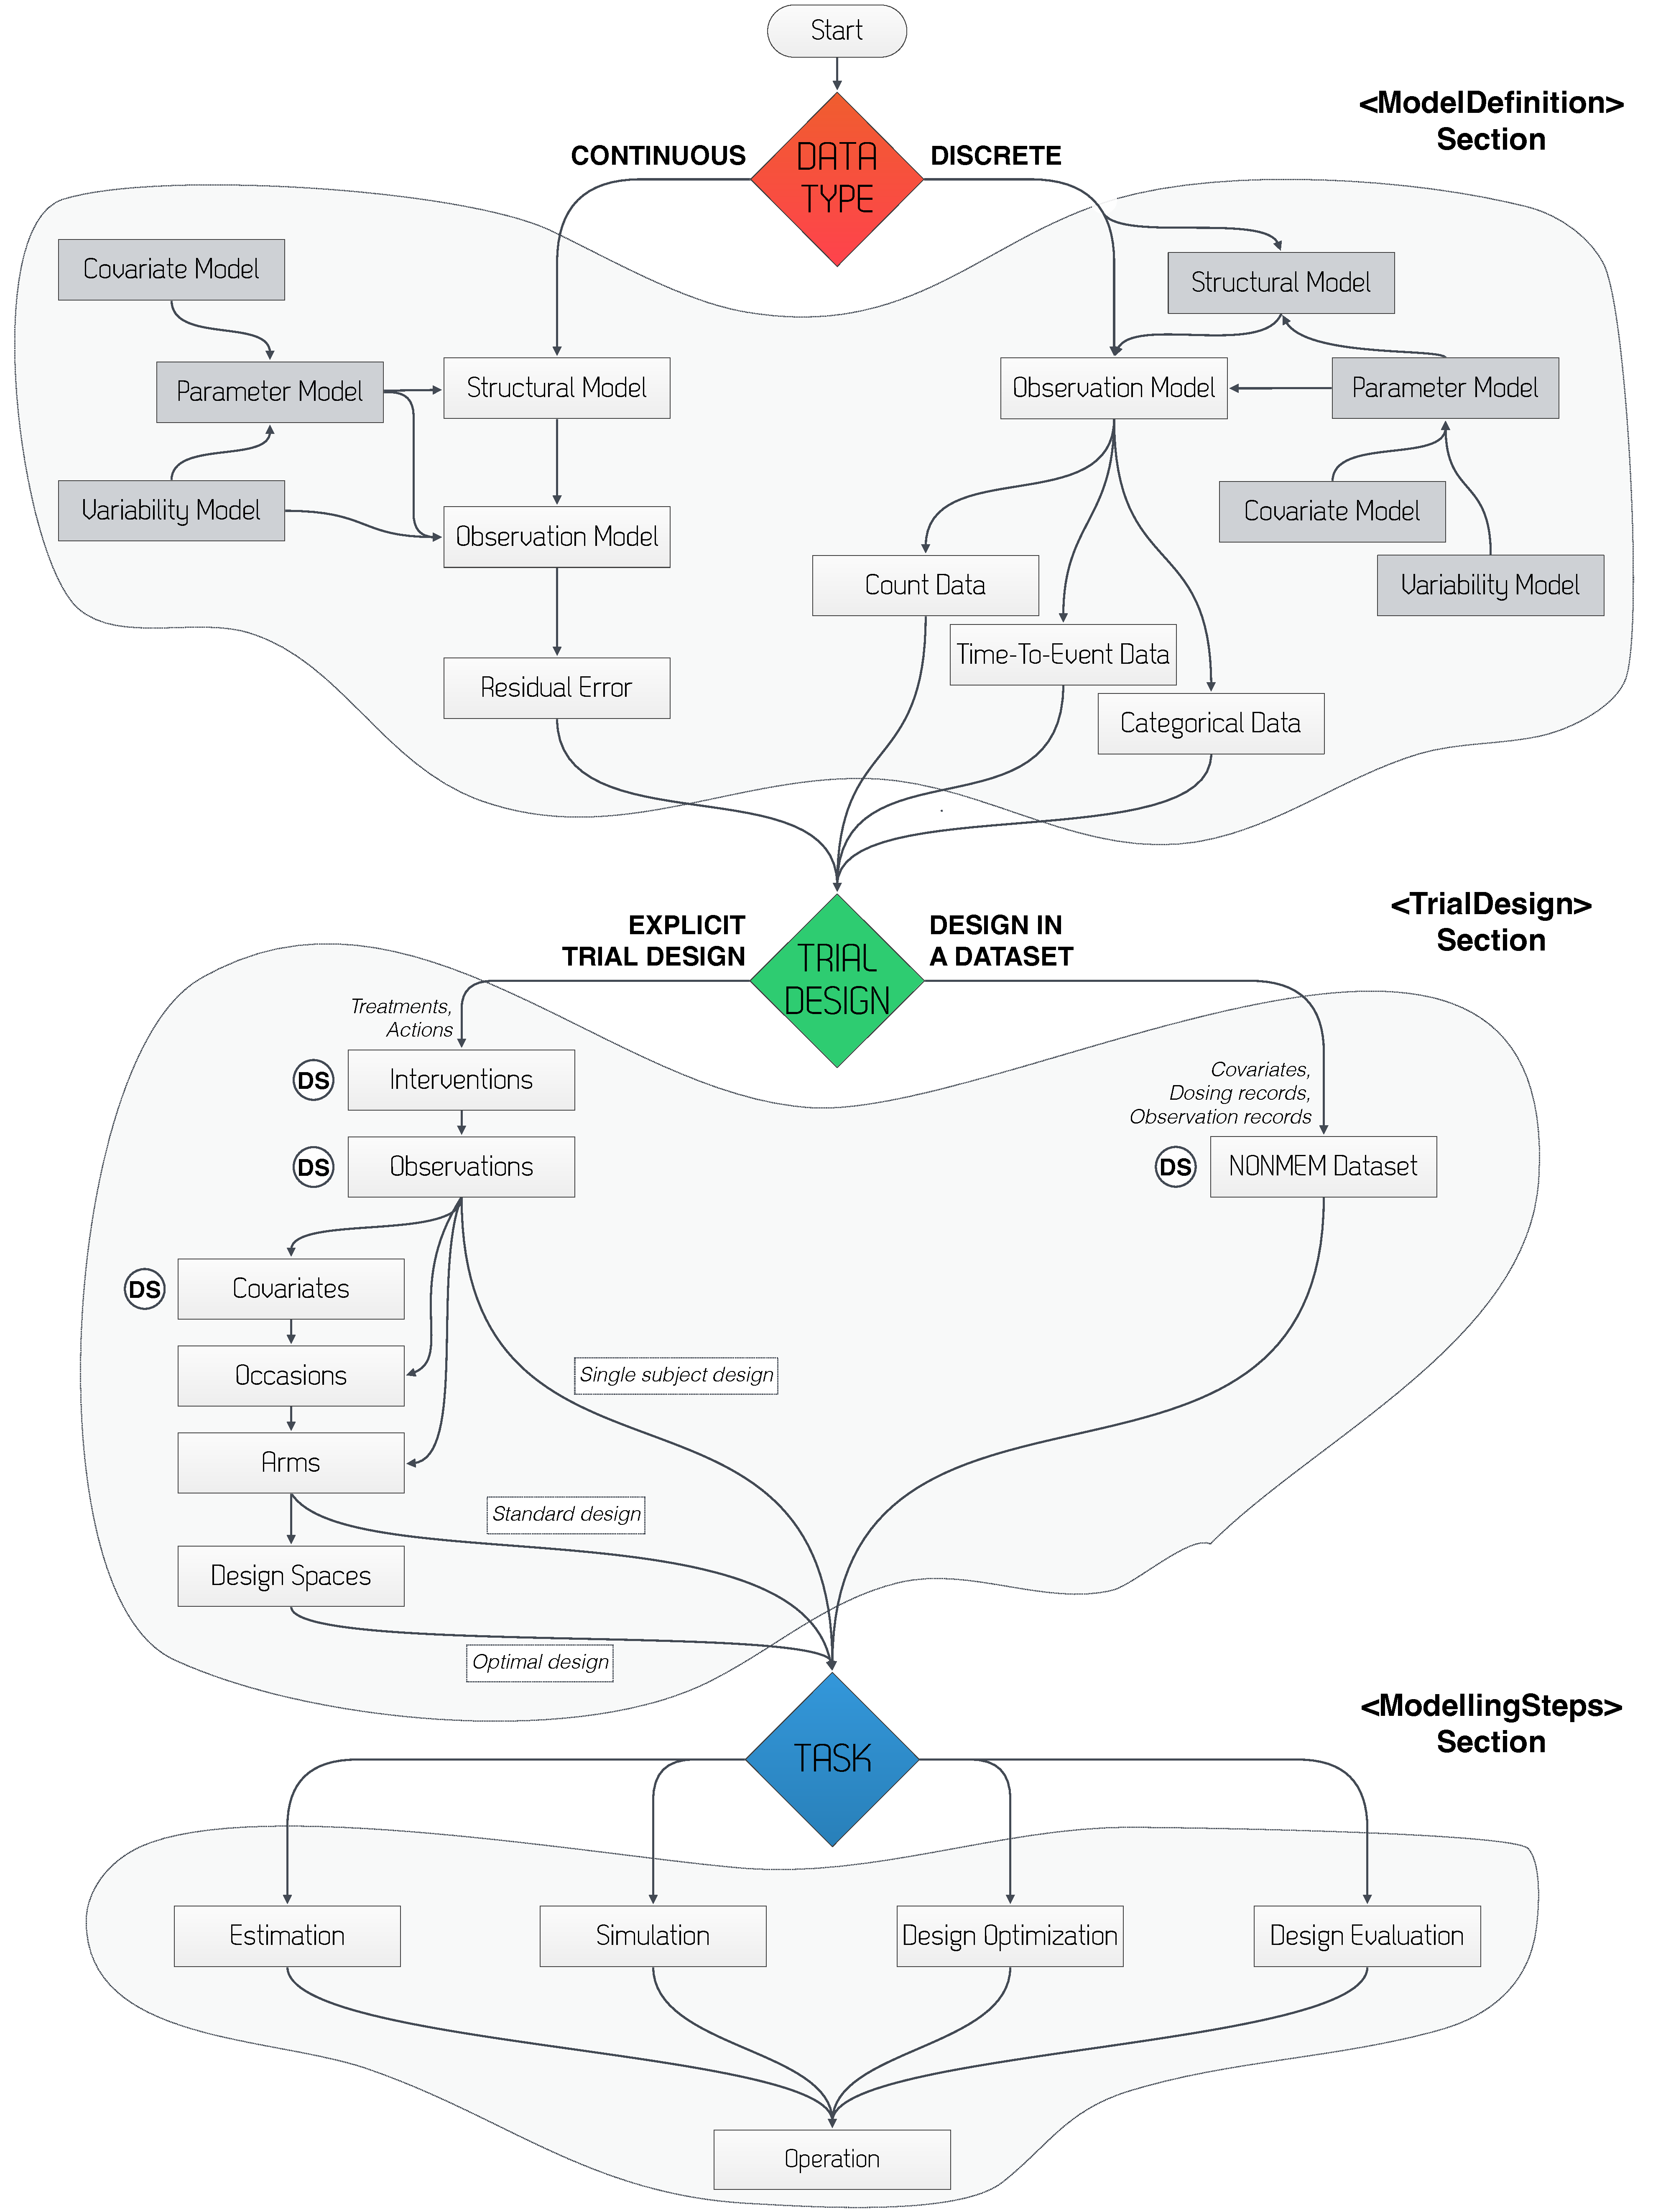
\includegraphics[width=90mm]{pics/Flowchart07}
\end{figure}



\vfill

% Bottom of the page
{\large \today \\}

\end{center}
\end{titlepage} 
\begin{titlepage}
\begin{center}

% Upper part of the page. The '~' is needed because \\
% only works if a paragraph has started.

\includegraphics[width=0.35\textwidth]{./logo/ddmore_logo}~\\[1cm]

%\textsc{\LARGE }\\[1.5cm]
%
\textsc{\Large Internal Release}\\[0.5cm]

% Title
\HRule \\[0.4cm]
{ \huge \bfseries Changes in PharmML 0.7.3 \\[0.4cm] }

\HRule \\[1.5cm]

% Author and supervisor
\begin{minipage}{0.75\textwidth}
\begin{flushleft} \large
Maciej J \textsc{Swat}\\
\emph{EMBL - European Bioinformatics Institute, Cambridge, UK} 
\end{flushleft}
\end{minipage}


\vfill



% Bottom of the page
{\large \today \\}

\end{center}
\end{titlepage} 

\linenumbers
\tableofcontents



%%%%%%%%%%%%%%%%%%%%%%%%%%%%%%%%%%%%%%%%%%%%%%%%%%%%%%%%%%%%%%%%%%%%%%
%%%%%%%%%%%%%%%%%%%%%%%%%%%%%%%%%%%%%%%%%%%%%%%%%%%%%%%%%%%%%%%%%%%%%%%
%%%%%%%%%%%%%%%%%%%%%%%%%%%%%%%%%%%%%%%%%%%%%%%%%%%%%%%%%%%%%%%%%%%%%%%
%%%%%%%%%%%%%%%%%%%%%%%%%%%%%%%%%%%%%%%%%%%%%%%%%%%%%%%%%%%%%%%%%%%%%%%
\chapter{Overview}
To avoid redundant and overlapping \marginpar{\HandCuffLeft} description this 
document contains only the changes in 0.7.3 version. For the detailed report on changes  
in PharmML 0.7--0.7.2 and ProbOnto 0.3, see the documents released with this version, 
\cite{Swat:2015b} and \cite{ProbOnto:2015a}.

\section*{Extensions/bug fixes in version 0.7.3}

\captionsetup[longtable]{skip=1em}
\LTcapwidth=\textwidth
\begin{center}
%\renewcommand{\arraystretch}{1.1}%
\begin{longtable}{lll}
\hline
\hline
\pml element 				&  version $\le$ 0.7.2 			& version 0.7.3 \\
or modelling aspect 			& 							& \\
\hline
\hline
Datasets, see section \ref{sec:ignore}& No support for ignoring records	& {\color{red} \scshape{new}} \xelem{IgnoreLine} \\[0.5ex]
\hline
Discrete data models,		& bug in PMF structure			& \xatt{linkFunction} renamed to the (optional) \\[-0.5ex]
see section \ref{sec:link}		&							& \xatt{transform} attribute \\ 	
\hline
\caption{Overview of major differences between versions $\le$ 0.7.2 and 0.7.3.}
\label{figTable:overviewTable4}
\vspace{-2em}
\end{longtable}
\end{center}



%%%%%%%%%%%%%%%%%%%%%%%%%%%%%%%%%%%%%%%%%%%%%%%%%%%%%%%%%%%%%%%%%%

\chapter{Changes in 0.7.3}
\label{ch:073changes}

\section{Commenting out of dataset records}
\label{sec:ignore}
Upon request within IOG, this version has been extended 
to support filtering out of rows in a datasets by allowing defining 
'ignore line' characters. For example $\#$ is often used for such 
purpose in NONMEM and Monolix-type datasets. 

These character(s) can contain up to three arbitrary characters 
without white spaces. The following snippet shows two such specifications, 
where the various symbols are defined, using <IgnoreLine> element, 
within the definition of the dataset, to identify rows to be omitted

\lstset{language=XML}
\begin{lstlisting}
    <DataSet xmlns="http://www.pharmml.org/pharmml/0.7/Dataset">
        <Definition>
            <Column columnId="TIME" columnType="idv" valueType="real" columnNum="1"/>
            <!-- skipped columns -->
            <Column columnId="MDV" columnType="mdv" valueType="int" columnNum="5"/>
            <IgnoreLine symbol="$10"/>
            <IgnoreLine symbol="#"/>
        </Definition>
        <ExternalFile oid="datasetID">
            <path>dataset.csv</path>
        </ExternalFile>
    </DataSet>
\end{lstlisting}
Any number of such 'ignore line' characters can be defined.

\section{\xatt{linkFunction} in discrete data models}
\label{sec:link}

The \xatt{linkFunction} attribute has been renamed to the (optional) \xatt{transform}
in the \xelem{PMF} element of the count data block. It was erroneously associated
with the probability mass function. Instead the transformation can be used to 
indicate that a transformed PMF has been encoded to be passed in such form to
a target tool, if supported. 

\paragraph{Example}
The common Poisson model can be implemented in its 
\begin{itemize}
\item 
default, untransformed form
\lstset{language=XML}
\begin{lstlisting}
<ObservationModel blkId="om1">
    <Discrete>
        <CountData>
            <CountVariable symbId="Y"/>
            <NumberCounts symbId="k"/>
            
	    <!-- P(Y=k) = (Lambda^k * exp(-Lambda) / k! -->
            <PMF>
                <math:LogicBinop op="eq">
                    <ct:SymbRef symbIdRef="Y"/>
                    <ct:SymbRef symbIdRef="k"/>
                </math:LogicBinop>
                <Distribution>
                    <po:ProbOnto name="Poisson1">
                        <po:Parameter name="rate">
                            <ct:Assign>
                                <ct:SymbRef symbIdRef="lambda"/>
                            </ct:Assign>
                        </po:Parameter>
                    </po:ProbOnto>
                </Distribution>
            </PMF>
\end{lstlisting}

\item 
in a log-transformed form
\lstset{language=XML}
\begin{lstlisting}
            <!-- log(P(Y=k)) = -Lambda+k*log(Lambda)-log(k!) -->
            <PMF transform="log">
                <math:LogicBinop op="eq">
                    <ct:SymbRef symbIdRef="Y"/>
                    <ct:SymbRef symbIdRef="k"/>
                </math:LogicBinop>
                <Distribution>
                    <po:ProbOnto name="Poisson1">
                        <po:Parameter name="rate">
                            <ct:Assign>
                                <ct:SymbRef symbIdRef="lambda"/>
                            </ct:Assign>
                        </po:Parameter>
                    </po:ProbOnto>
                </Distribution>
            </PMF>
\end{lstlisting}

\item 
or in log-transformed explicit form
\lstset{language=XML}
\begin{lstlisting}
            <!-- explicit log(PMF) -->
            <!-- log(P(Y=k)) = -Lambda+k*log(Lambda)-log(k!) -->
            <PMF transform="log">
                <math:LogicBinop op="eq">
                    <ct:SymbRef symbIdRef="Y"/>
                    <ct:SymbRef symbIdRef="k"/>
                </math:LogicBinop>
                <ct:Assign>
                    <math:Binop op="minus">
                        <math:Binop op="plus">
                            <math:Uniop op="minus">
                                <ct:SymbRef blkIdRef="pm1" symbIdRef="lambda"/>
                            </math:Uniop>
                            <math:Binop op="times">
                                <ct:SymbRef symbIdRef="k"/>
                                <math:Uniop op="log">
                                    <ct:SymbRef blkIdRef="pm1" symbIdRef="lambda"/>
                                </math:Uniop>
                            </math:Binop>
                        </math:Binop>
                        <math:Uniop op="factln">
                            <ct:SymbRef symbIdRef="k"/>
                        </math:Uniop>
                    </math:Binop>
                </ct:Assign>
            </PMF>
        </CountData>
    </Discrete>
</ObservationModel>
\end{lstlisting}
\end{itemize}
Note, that the last implementation should be used only if a certain 
distribution is not covered by ProbOnto/UncertML. It is the option allowing
the implementation of an arbitrary user-defined distributions.






%\bibliographystyle{abbrvnat}
\bibliographystyle{myplainnat}
\bibliography{pharmml-specification}
\end{document}
